\documentclass{article}
\usepackage{graphicx} % Required for inserting images
\usepackage{outlines}
\usepackage{svg}
\usepackage{wrapfig}
\usepackage{tikz}
\usepackage{url}

%Here is an updated draft project proposal incorporating the MOU between SAHA and TMM as well as the medication budget for the NCD outreach campaign:

%Title: Improving NCD Care Delivery in Somaliland through Outreach and OpenEMR

%\title{NCD Campaign in Somaliland \\
%Taiwan Medical Mission (Project)}
%\author{Dr. Tex Li-Hsing Chi}
%\date{\today}

\begin{document}


\begin{titlepage}
%    \centering

%\begin{center}
\hspace*{-0.7cm}%
\begin{tikzpicture} % tikzfigure
%\begin{minipage}[b]{1\linewidth}

\includesvg[height=3.0cm, distort=false]{Flag_of_the_Republic_of_China.svg}
\hspace{1.4cm}
%\includesvg[width=0.17\linewidth]{TMM_logo.svg}
%\hspace{3cm}
\includesvg[height=3.0cm, distort=false]{Flag_of_Somaliland.svg}
%\captionof{Figure}{xx}
%\end{minipage}
\end{tikzpicture}
    \vspace{2cm}
    
\centering
    {\Huge\bfseries Taiwan---Somaliland \\
    Bridging Borders,\\ Mending Bones  \par } % \\
 %   Handbook\par}
    \vspace{1.5cm}
    %\hspace{4cm} 
    {\Large October 2023\par}

%\end{center}

\vspace{2.0cm}
%\includesvg[height=3.5cm, distort=false]{TMWH_logo(noWord).svg}


\vspace{1.5cm}
\includesvg[height=2.9cm, distort=false]{logo_MoHD_HGH.svg}

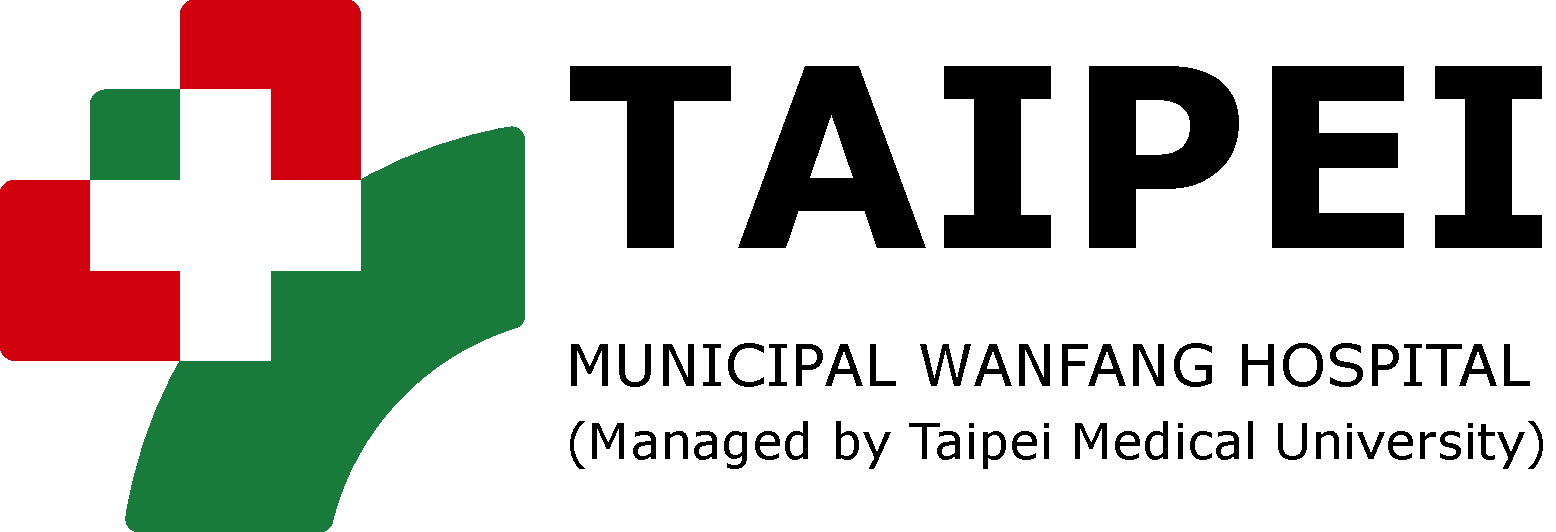
\includegraphics[height=1.8cm]{TMWH_logo_TAIPEI_vector.pdf}
\includesvg[height=2.1cm, distort=false]{HGH_orthopedic_logo.svg}
\includesvg[height=2.2cm, distort=false]{HGH_neurosurgery_logo.svg} 


%\vspace{1cm}


\end{titlepage}



%\hfill
%\begin{wrapfigure}[1]{l}{0.0\linewidth}%{height=0.65\textheight}
%    \centering
%    \includesvg[width=0.20\textwidth]{TMM_logo.svg}
%\end{wrapfigure}
%\vspace{1.5cm}

%\maketitle

\noindent
\begin{minipage}{0.2\textwidth}
\centering
\includesvg[width=0.9\linewidth]{TMM_logo.svg}
\end{minipage}
\hfill
\begin{minipage}{0.75\textwidth}
\centering
{\LARGE\bfseries TMM---HGH Project \\ 
Save LIVES \\ For World Trauma Day \\
- Bone Health Campaign }\\[1ex]
\large\textit{Dr. Tex Li-Hsing Chi}\\[2ex]
\today
\end{minipage}


%%%
\section{Background}
Taiwan Medical Mission (TMM) aims to build medical capacity in the Republic of Somaliland through specialty training exchanges, outreach programs, and visiting scholar opportunities at Hargeisa Group Hospital (HGH).
% , and developing equipment maintenance capabilities

TMM has identified focus areas for 2024, including hemodialysis, critical care, orthopedics, non-communicable diseases (NCDs), nursing, telemedicine, visiting specialists, outreach campaigns, and establishing a visiting scholar program for HGH staff to train in Taiwan.

Key initiatives planned for 2024 are:

\begin{itemize}
%\item Hemodialysis - AV fistula surgery training, tele-nephrology conferences
\item Critical care - local and Taiwan ICU training
\item Orthopedics - local and Taiwan orthopedic surgeon training
%\item NCD clinic - partnership with NGO SAHA on NCD prevention
%\item Nursing fundamentals training program
\item Visiting specialists - Taiwanese specialists performing surgeries and training
\item Telemedicine for case discussions and virtual consults
%\item Teleradiology and telepathology platforms
\item Outreach campaigns on orthopedic/trauma, oral health, eye care, blood donation, and osteoporosis awareness
\item Visiting scholar program for HGH staff to train in Taiwan
%\item Procurement of medical equipment and maintenance training
\end{itemize}

%To support these initiatives, TMM has proposed a 
%budget of around USD 442,000 for 2024. This includes funding for relief supplies, visiting scholar program, equipment, transportation, and program activities.
% , upgrade equipment and maintenance capabilities,

%The goal is to exchange specialty knowledge, expand access to care, and improve public health outreach. This will build local capacity at HGH through collaboration between Somaliland and Taiwanese healthcare professionals.

To support capacity-building initiatives at Hargeisa Group Hospital, TMM has proposed an \textbf{Orthopedic and Trauma Surgery Collaboration and Outreach project} for 2023. 
This will enable knowledge exchange between Taiwanese orthopedic specialists and Somalilander surgeons. Orthopedics was a priority area because musculoskeletal injuries and conditions are highly prevalent, often requiring surgical intervention. With road traffic accidents being a significant cause of injury in Somaliland, improving local trauma surgery capabilities will save lives and prevent disabilities. The outreach component will also increase public awareness of injury prevention, first aid, and bone health. By facilitating hands-on training, virtual learning, and community outreach focused on orthopedic care, this initiative will significantly advance local capabilities while providing life-changing treatment to needy patients.


%%
\section{Objectives}
\begin{outline}
\1 To perform complex orthopedic or neurosurgery procedures, including fracture surgery, arthroscopic surgery, and spine surgery during \textbf{Dr. Kuo's visit}.
\1 To provide training and demonstration for local orthopedic surgeons on techniques and approaches.
\1 To increase access to orthopedic surgical care for patients in Somaliland.
\1 To promote community injury prevention and first aid awareness through outreach around \textbf{Save LIVES for World Trauma Day on October 17}.

%\1 To raise awareness of bone health and risks of vitamin D deficiency in women for \textbf{World Osteoporosis Day on October 20}.
% reasons for postpone it:
%Here are my thoughts on the questions about the outreach campaigns:
%1) Based on the holiday on 10/20, I would recommend focusing on the World Trauma Day outreach on 10/17 during Dr. Kuo's visit. This avoids overlap with the holiday closure.
%2) I agree transforming the Trauma Day outreach into a surgical campaign to treat injuries patients for free would be impactful. The awareness component could still be incorporated through education while patients are awaiting or recovering from surgery. 
%3) Given the short timeline until 10/20 and need to procure supplies, it makes sense to postpone the Osteoporosis Day outreach to a future date when there is more preparation time. The Trauma Day surgical camp will already capture many injury/fracture patients who are at risk of osteoporosis.
%In summary, my suggestions would be:
%- Focus on Trauma Day surgical outreach from 10/16-30 during Dr. Kuo's visit 
%- Postpone Osteoporosis Day outreach to a future date when supplies can be arranged
%- Combine awareness messaging for both causes into the Trauma Day camp (injury prevention and bone health education)
%Please let me know if you have any other questions! I'm happy to discuss further.

\end{outline}


\section{Activities}

\begin{outline}
\1 Orthopedic and neurosurgery procedures will be performed by Dr. Kuo and local surgeons at Hargeisa Group Hospital from October 16-30, including:
\2 Arthroscopic surgery
\2 Spine surgery
\2 Proximal femoral fracture surgery

\1 Observation and cooperation by Dr. Ahmed, Dr. Hassan, orthopedic residents, and neurosurgeons Dr. Abdulhamid and Dr. Mustafe.
%\1 Use of C-arm x-ray imaging assistance
\1 Training sessions and case reviews for knowledge exchange

\1 Outreach event for World Trauma Day on October 17:
\2 Host awareness rally on injury prevention and first aid
\2 Educate the public on WHO road safety initiatives and interventions
\2 Provide basic life support (BLS) training

%\1 Outreach event for World Osteoporosis Day on October 20 (Friday):
%\2 Education and awareness activities on bone health
%\2 Free vitamin D blood tests for women
%\2 Bone density screening
\end{outline}
%%%
\clearpage

%Here is a section on the OPD settings:

\section{Operation Settings}
The orthopedic procedures will occur in the operating theater at Hargeisa Group Hospital, led by Dr. Ahmed and Dr. Kuo, with cooperation from orthopedic resident Dr. Hassan.
Dr. Kuo and neurosurgeons (Dr. Mustafe and Dr. Abdulhamid) will conduct the spine procedures. %C-arm x-ray imaging will be used as needed during surgery
Dr. Kuo's background in advanced spine surgery techniques will be very beneficial for exchanging knowledge and enhancing local capabilities in treating complex spine conditions through minimally invasive and endoscopic approaches. His expertise nicely complements the neurosurgical spine capabilities at HGH.

%
\subsection{Surgery Categories}

\begin{outline}
\1 Surgeries led by Dr. Ahmed and Dr. Kuo, orthopedic surgeons

\1 Neurosurgical cooperation for spine procedures by Dr. Mustafe and Dr. Abdulhamid:

    \2 Spine fixation for thoracolumbar fractures using pedicle screws
    \2 Lumbar disk herniation treatment
    \2 Cervical spine fusion for degenerative changes or unstable fractures

\1 Dr. Kuo also brings extensive spine surgery expertise:

    \2 Degenerative spine disease treatment - cervical, lumbar
    \2 Intervertebral disc herniation
    %\2 Spine surgery - corrective, minimally invasive, endoscopic
    \2 Scoliosis
    \2 Spinal tumor
    \2 Vertebral fracture
    \2 Spinal infection

\1 Use of C-arm X-ray imaging during surgery for joints

\1 Post-operative care in orthopedic or neurosurgery ward

\1 Follow-up in orthopedic or neurosurgery OPD
\end{outline}





%%
\subsection{Workflow for Patients}

\begin{outline}
\1 Patient source: orthopedic or neurosurgery outpatient department
\2 Pre-operation assessment
\2 Admission process on the day before surgery

\1 Operation day:
\2 Patient prepared in the pre-op area
\2 Surgery performed in OT
\2 Post-op recovery in OT
\2 Transfer to the orthopedic or surgical inpatient ward

\1 Post-op care inwards:
\2 Vitals monitoring
\2 Pain management
\2 Mobilization and physical therapy
\2 Wound care
\2 Discharge planning

\1 Follow-up at OPD after discharge

\end{outline}

%%



\clearpage
%%%%%%%%%%%%%%5
\section{Outreach Settings}
The World Trauma Day awareness rally and activities on October 17 will be hosted at a public venue in Hargeisa Group Hospital. % a kick-off ceremony with DG Dr. Hergeye and TRO
%The World Osteoporosis Day events on October 20 will take place at Hargeisa Group Hospital.

During Dr. Kuo's visit, the World Trauma Day surgical outreach camp will occur from October 16-30 at Hargeisa Group Hospital. 
This will provide free spine or orthopedic surgery for injured patients.

%\begin{outline}
%For a \textbf{multi-day} The World Osteoporosis Day at Hargeisa Group Hospital:

%\1 Outreach conducted annually
%\1 Site selection by demand: Boroma, Berbera, Burco, or around other cities
%\1 Outreach hours: 08:00 - 17:00 for the first few days, 08:00 - 13:00 on the last day
%\end{outline}

\subsection{Outreach Preparation}

\begin{outline}
%    \1 Application of outreach approval from the Ministry of Health Development (MoHD)
    \1 Assemble the outreach team and assign roles
    \1 Gather equipment and supplies
    \1 Print patient forms and educational materials
%    \1 Team members' access to food, water, transportation, and security

\end{outline}

\subsection{Community Outreach}


\begin{outline}
To use local channels and networks to reach people:

\1 Use social media like Facebook, Twitter, and Instagram to share information, photos, and videos.

\1 Distribute flyers, posters, and banners in markets, mosques, schools, and clinics.

\1 Ask leaders and volunteers to spread the word.

\1 Send SMS reminders about dates, location, and registration.

\1 Partner with local TV stations to broadcast announcements.

\1 Use community health workers to gather and register people.

\1 An official ceremony to announce \textbf{Word Traum Day} campaign during 16-30 October 2023
    \2 For Injury prevention and first aid training (trauma focus)
    \2 Bone health education (osteoporosis focus)
    \2 Messaging will underscore the relationship between traumatic injuries, fractures, and longer-term risks like osteoporosis. Education will empower the community to take action to protect bone health across the lifespan.
\end{outline}


%\subsection{Outreach Schedule}
%An ENT campaign (i.e., operation for Tonsillitis) in Hargeisa, Somaliland, in August 2023:
%According to one-day campaign:

%\begin{outline}
%For one-day outreach activity schedule in Hargeisa:
%	\1 08:00 - Set up screening stations

%    \1 08:30 - Patients start arriving

%    \1 09:00 - Screenings and consultations start

%    \1 10:00 - Patient education sessions

%    \1 11:00 - Wrap up screening and consultations

%    \1 12:20 - Break down stations

%    \1 13:00 - Depart
%\end{outline}
%


%%%

\section{Expected Outcomes}

% By combining education on both injury prevention and bone health, the camp will take advantage of the synergies between traumatic injuries and osteoporosis. This dual messaging will maximize the impact and value for the community.
\begin{outline}
\1 For medical staff:
\2 Completion of complex spine or orthopedic surgeries to treat patients
\2 Enhanced surgical skills and knowledge among local orthopedic team

\1 For patients:
\2 Provide free orthopedic and neurosurgery for injured patients
\2 Increased public awareness of injury prevention and first aid
\2 Improve understanding of lifelong bone health and osteoporosis risks
%\1 Identification of vitamin D deficiency and osteoporosis cases through screening
\end{outline}

%%%%%%%%%%%%%%%%%

\section{Challenges and Solutions}
With strong collaboration, planning, and adaptable implementation, the challenges can be overcome to make the initiatives successful.

\begin{outline}

%\1 Limited surgical equipment and supplies
%\2 Partner with TMM for procurement of essential tools, implants, consumables

%\1 Infrastructure limitations in OT
%\2 Optimize existing infrastructure, explore facility upgrades

%\1 Shortage of trained surgical staff
%\2 Hands-on training by Dr. Kuo, virtual learning, visiting scholar program

%\1 Referral delays for complex cases
%\2 Streamline referral process, utilize telemedicine for prompt consultations

\1 Limited public awareness of trauma/bone health
\2 Engaging outreach with clear educational messaging

\1 Transportation barriers for patients
\2 Arrange logistics support for those in need

\1 Post-op care coordination
\2 Cross-training nurses, protocols to facilitate care transitions

%\1 Data limitations for monitoring
%\2 Implement tracking logs to collect key metrics

\end{outline}



%%
\clearpage

\section{(draft) Budget Planning}
Costs to include:
\begin{outline}
\1 Surgical equipment and supplies, especially diathermy machine in HGH OT
\1 Arthroscopic instruments (to be installed in HGH OT in February 2023)
\1 C-arm x-ray instruments (to be installed in HGH OT in August 2023)
%\1 Venue and logistics for outreach events
\1 Printed educational materials
%\1 Vitamin D test kits
%\1 Bone density screening machine
\end{outline}

%Total: USD 10,000



%\section{Reference}
%(1) Interpreting the Lancet surgical indicators in Somaliland: a cross-sectional study. https://bmjopen.bmj.com/content/10/12/e042968 Accessed 11/05/2023.
%(2) ENT Department | Somali Sudanese specialized hospital. ENT Department | Somali Sudanese specialized hospital (ssshospital.so) Accessed 11/05/2023.


\end{document}
